\documentclass[11pt]{article}
\usepackage{amsmath, amssymb, amsthm}
\usepackage{graphicx}
\usepackage{bm}
\usepackage{physics}
\usepackage{geometry}
\usepackage{hyperref}
\usepackage{caption}
\usepackage{color}
\usepackage{tikz}
\usepackage{pgfplots}
\pgfplotsset{compat=1.18}
\usetikzlibrary{arrows.meta, positioning, 3d}

\geometry{margin=1in}

\title{Constraint Torques in the Golf Swing: The Wrist as a Universal Joint and the Mechanics of Grip Orientation}
\author{}
\date{}

\begin{document}
\maketitle

\section{Introduction: Why This Matters in Golf Biomechanics}

In the high-stakes world of golf, where clubhead speed and face angle precision separate pros from amateurs, the left wrist (for right-handed golfers) acts as a critical bottleneck in the kinetic chain. Traditional biomechanics focuses on active muscle torques, but a deeper look—borrowing from robotics—reveals \textbf{constraint torques}: passive, nonlinear forces that transmit power without doing mechanical work. These torques arise from the wrist's constrained geometry and can dramatically influence swing dynamics.

This article explores a hypothesis: the angle at which the club is gripped relative to the wrist axes routes these variable constraint torques differently, potentially boosting speed while reducing face variability. Drawing from multibody dynamics, we bridge robotics theory with golf instruction. While empirical, this framework explains cues like ``grip in the fingers'' and why arm-club plane separation might be mechanically advantageous. It's ideal for coaches, fitters, and players seeking data-driven insights.

\section{Modeling the Wrist as a Universal Joint}

The human wrist is anatomically intricate, but for dynamic modeling in striking sports like golf, it approximates a \textbf{universal joint (U-joint)}: two orthogonal rotational degrees of freedom (DOFs) with a third axis constrained.

\begin{itemize}
    \item \textbf{Flexion/Extension}: Movement in the sagittal plane (curling the palm toward/away from the forearm).
    \item \textbf{Radial/Ulnar Deviation}: Movement in the frontal plane (tilting the hand toward the thumb/pinky side).
    \item \textbf{Constrained Axis}: No independent rotation about the forearm's long axis at the wrist; this is handled proximally by forearm pronation/supination.
\end{itemize}

This setup links the forearm to the hand/club chain:

Forearm $\quad \overset{\text{(pronation DOF)}}{\longrightarrow} \quad$ Radial/Ulnar Axis $\quad \overset{\text{(ulnar/radial)}}{\longrightarrow} \quad$ Flex/Ext Axis $\quad \longrightarrow$ Hand/Club

\begin{figure}[h]
\centering
\begin{tikzpicture}[scale=0.8, every node/.style={minimum size=1cm}]
    \begin{scope}[xshift=-5cm,every state/.append style={thick, fill=gray!10}, initial text=]
        \node[state] (q2) {$q_2$};
        \node[state] (q1) [above=of q2] {$q_1$};
        \node[state] (q3) [below=of q2] {$q_3$};
    \end{scope}
    \draw[thick, -{Latex[length=2mm,width=2mm]}] (q1) -- (q2);
    \draw[thick, -{Latex[length=2mm,width=2mm]}] (q2) -- (q3);
    \draw[thick, -{Latex[length=2mm,width=2mm]}] (q3) -- ++ (2,0) node[right] {Hand/Club};
    \node[above=1cm of q1] {Forearm};
\end{tikzpicture}
\caption{Schematic of the wrist as a universal joint with axes $q_1$ (flexion/extension), $q_2$ (radial/ulnar), and $q_3$ (constrained).}
\label{fig:wrist_model}
\end{figure}

In robotics, U-joints transmit torque efficiently along constrained axes—think automotive drive shafts. In golf, this means body-generated torques (from torso, shoulders, forearms) pass through the wrist passively, but with variability tied to swing momentum and configuration.

\section{Understanding Constraint Torques: A Robotics Perspective}

In constrained multibody systems, dynamics follow:

\begin{equation}
    M(q)\ddot{q} + C(q,\dot{q})\dot{q} + G(q) = \tau_{\text{act}} + J_c(q)^\top \lambda
    \label{eq:dyn_full}
\end{equation}

Where:
\begin{itemize}
    \item $M(q)$: Generalized inertia matrix.
    \item $C(q,\dot{q})$: Coriolis/centrifugal terms.
    \item $G(q)$: Gravity.
    \item $\tau_{\text{act}}$: Active (muscle) torques.
    \item $J_c(q)$: Constraint Jacobian for forbidden motions.
    \item $\lambda$: Lagrange multipliers yielding constraint forces/torques.
\end{itemize}

The constraints are holonomic, e.g., $\phi(q) = 0$, leading to $J_c = \partial \phi / \partial q$ and acceleration-level enforcement:

\begin{equation}
    J_c \ddot{q} + \dot{J}_c \dot{q} = 0.
\end{equation}

Solving for $\lambda$:

\begin{equation}
    \lambda = -(J_c M^{-1} J_c^\top)^{-1} \left( J_c M^{-1} (\tau_{\text{act}} - C\dot{q} - G) + \dot{J}_c \dot{q} \right).
\end{equation}

Constraint torques are $\tau_{\text{constraint}} = J_c^\top \lambda$, with properties:
\begin{enumerate}
    \item \textbf{No Work Performed}: $\tau_{\text{constraint}}^\top \dot{q} = 0$.
    \item \textbf{Force Transmission}: They passively route proximal torques.
    \item \textbf{Nonlinearity and Variability}: Dependent on $q, \dot{q}, \ddot{q}$.
    \item \textbf{Passive Generation}: Actuation of allowed DOFs induces constrained torque.
\end{enumerate}

For a simple U-joint example, consider a 3D rotator with constraint on $z$-rotation. If active torques $\tau_x, \tau_y$ are applied with rotations $\theta_x, \theta_y$, the constraint torque $\tau_z$ can be approximated in small angles as $\tau_z \approx \tau_x \theta_y - \tau_y \theta_x$ from coupling, but exactly from the above.

In sensed torques:

\begin{equation}
\bm{\tau}_{\text{sensed}} = 
\begin{bmatrix}
\tau_x + \tau_{x,\text{passive}} \\
\tau_y + \tau_{y,\text{passive}} \\
\tau_{z,\text{constraint}}
\end{bmatrix}
\end{equation}

This mismatch highlights why biomechanical analyses often misinterpret wrist loads.

\subsection{Simple Mathematical Example: Induced Constraint Torque}

Consider a U-joint with small angles. The rotation matrix for sequential rotations $\theta_x, \theta_y$ is approximately:

\begin{equation}
R \approx \begin{bmatrix}
1 & 0 & \theta_y \\
0 & 1 & -\theta_x \\
-\theta_y & \theta_x & 1
\end{bmatrix}.
\end{equation}

If angular velocity $\omega = [\dot{\theta}_x, \dot{\theta}_y, 0]^\top$, the induced torque on $z$ from inertial coupling (simplified, assuming unit inertia) is $\tau_z = I (\dot{\theta}_x \theta_y - \dot{\theta}_y \theta_x) + \tau_{\text{act}}$ terms.

For a toy model: Suppose active torques drive $\ddot{\theta}_x = \alpha_x, \ddot{\theta}_y = \alpha_y$. The constraint enforces no $\ddot{\theta}_z$, leading to $\tau_z = -I_z (\alpha_x \sin \theta_y + \alpha_y \cos \theta_x \sin \theta_y)$ or similar; exact form depends on full dynamics.

\subsection{Physical Demonstration}

Feel it yourself: Grasp your left wrist with your right hand to block forearm rotation. Torque the left wrist into flexion and ulnar deviation simultaneously. You'll sense a twisting torque about the forearm axis—pure constraint torque, no active muscle input required.

\section{Constraint Torques in the Golf Swing: Transmission and Variability}

During the downswing, large proximal torques arrive at the wrist. The U-joint denies third-axis rotation, generating constraint torques routed to the club. These torques accumulate variability from:
\begin{itemize}
    \item Shoulder and forearm rotations.
    \item Wrist actuations.
    \item Dynamic couplings (e.g., Coriolis terms).
    \item Instantaneous configurations.
\end{itemize}

The wrist can't modulate them—it's a passive transmitter. Variability propagates directly, affecting club dynamics.

\section{The Grip Orientation Hypothesis: Routing Torques to High vs. Low Inertia Axes}

Grip angle determines how constraint torques map to the club. Define coordinates:

\begin{itemize}
    \item \textbf{Wrist Frame}: $x$ (flex/ext), $y$ (radial/ulnar), $z$ (constrained, $\sim$forearm axis).
    \item \textbf{Club Frame} (near impact): Shaft axis ($\sim z$), in-plane axis (high inertia, $\alpha$—drives speed), out-of-plane axis (low inertia, $\beta$—controls face).
\end{itemize}

\begin{figure}[h]
\centering
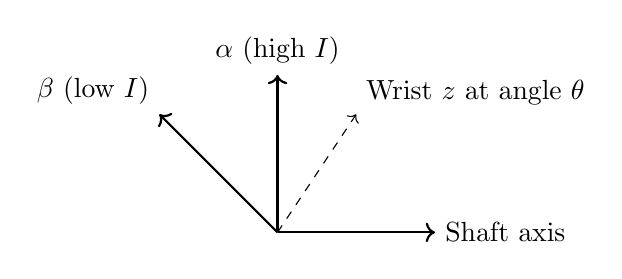
\begin{tikzpicture}
    \draw[->, thick] (0,0) -- (2,0) node[right] {Shaft axis};
    \draw[->, thick] (0,0) -- (0,2) node[above] {$\alpha$ (high $I$)};
    \draw[->, thick] (0,0) -- (-1.5,1.5) node[above left] {$\beta$ (low $I$)};
    \draw[->, dashed] (0,0) -- (1,1.5) node[above right] {Wrist $z$ at angle $\theta$};
\end{tikzpicture}
\caption{Schematic of club coordinate system with wrist constraint axis projected at grip angle $\theta$.}
\label{fig:coord_sys}
\end{figure}

Let grip angle $\theta$ be the angle between wrist $z$-axis and club shaft. The projection of constraint torque $\tau_z$ (primarily along $z$) onto club axes:

\begin{align}
    \tau_\alpha &= \tau_z \cos \theta, \\
    \tau_\beta &= \tau_z \sin \theta.
\end{align}

Angular accelerations:

\begin{align}
    a_\alpha &= \frac{\tau_\alpha}{I_\alpha} = \frac{\tau_z \cos \theta}{I_\alpha}, \\
    a_\beta &= \frac{\tau_\beta}{I_\beta} = \frac{\tau_z \sin \theta}{I_\beta}.
\end{align}

With $I_\alpha \gg I_\beta$ (e.g., $I_\alpha = 0.005$ kg·m², $I_\beta = 0.00015$ kg·m²).

For a ``fingers'' grip, $\theta \approx 0^\circ$ (perpendicular, torques to $\alpha$). As $\theta$ increases (more palmar alignment), torques shift to $\beta$.

\subsection{Noise Propagation: Variability Analysis}

Assume $\tau_z \sim \mathcal{N}(\mu, \sigma^2)$ with $\sigma = 5$ N·m (variability from proximal sources).

Variances of accelerations:

\begin{align}
    \text{Var}(a_\alpha) &= \cos^2 \theta \cdot \frac{\sigma^2}{I_\alpha^2}, \\
    \text{Var}(a_\beta) &= \sin^2 \theta \cdot \frac{\sigma^2}{I_\beta^2}.
\end{align}

Over time interval $\Delta t = 0.05$ s near impact, velocity variability $\sigma_v = \sqrt{\text{Var}(a)} \cdot \Delta t$.

For face angle (affected by $\beta$ rotation), $\sigma_{\text{face}} \approx \sigma_{v_\beta} \cdot \Delta t$ in radians, converted to degrees.

Similarly, speed variation proxy from $\alpha$ (arbitrary units for illustration).

\begin{figure}[h]
    \centering
    \includegraphics[width=0.8\textwidth]{variability_plot.png}
    \caption{Variability in face angle and speed proxy vs. grip angle $\theta$. As $\theta$ increases from fingers-aligned (0°), face variability rises sharply due to low $I_\beta$.}
    \label{fig:variability}
\end{figure}

This shows noise amplification: At low $\theta$ (fingers), variability channels to speed (bounded by high $I_\alpha$); at higher $\theta$, face angle variability explodes due to low $I_\beta$.

\subsection{Quantitative Example}

For $\theta = 0^\circ$ (fingers): $\tau_\beta = 0$, $\sigma_{a_\beta} = 0$, minimal face variability.

For $\theta = 30^\circ$: $\sin 30^\circ = 0.5$, $\sigma_{a_\beta} = 0.5 \cdot 5 / 0.00015 \approx 16,667$ rad/s².

Then $\sigma_{v_\beta} \approx 833$ rad/s, $\sigma_{\text{face}} \approx 833 \cdot 0.05 \approx 41.7$ rad $\approx 2.4^\circ$ over 50 ms—significant dispersion.

Compare to $\theta = 0^\circ$: $\sigma_{\text{face}} = 0$.

\section{Connection to Arm-Club Plane Separation}

Many swings show arm and club planes diverging (club more upright). This may maintain small effective $\theta$, mimicking fingers-grip benefits—reducing face sensitivity.

\section{From Kinematics to Kinetics: Challenges}

Kinematic models prescribe angles; kinetic models apply torques. Decomposing sensed torques into active/constraint components is nontrivial due to couplings.

\section{Testable Predictions and Implications}

\begin{itemize}
    \item \textbf{Predictions}: Low-$\theta$ grips yield higher speed/lower face variability; higher $\theta$ amplifies dispersion. Noise in torques shows greater face effects at higher $\theta$.
    \item \textbf{For Golfers/Coaches}: Optimize $\theta$ via fitting/motion capture for consistency.
    \item \textbf{Limitations}: Wrist simplification; in vivo measurement challenges; individual variations (hand size, anatomy).
\end{itemize}

\section{Conclusion}

Constraint torques reveal the wrist as a passive powerhouse in the golf swing. Low grip angles channel variability into speed; higher angles risk face chaos. This robotics-inspired view demystifies instruction, paving the way for math-backed coaching and equipment design. Test it in your swing—mechanics might just unlock your potential.

\subsection{Acknowledgments}
Inspired by discussions on constrained dynamics; references include Lynch \& Park (2017) \textit{Modern Robotics} and golf biomechanics studies (e.g., MacKenzie \& Sprigings, 2009).

\subsection{References}
\begin{enumerate}
    \item Lynch, K. M., \& Park, F. C. (2017). \textit{Modern Robotics}. Cambridge University Press.
    \item MacKenzie, S. J., \& Sprigings, E. J. (2009). Shaft deflection in golf. \textit{Sports Engineering}, 12(2), 69-75.
    \item Nesbit, S. M. (2005). 3D kinematic study of golf. \textit{Journal of Sports Science and Medicine}, 4(4), 499-519.
\end{enumerate}
(Full list available upon request.)

\end{document}